\subsection{Fabric interface}

Address bus can have one of the following values:
\begin{center}
\begin{tabular}{|c|l|}
  \hline {\bf decimal value} & {\bf meaning of data word on data bus}\\
  \hline
  \emph{0} & regular data (packet header and payload)\\
  \emph{1} & OOB (Out-of-band) data\\
  \emph{2} & status word\\
  \emph{3} & currently not used\\
  \hline
\end{tabular}
\end{center}

{\bf Status word} (sent when the value of address bus is \emph{2}) contains
various information about Ethernet frame's structure and type:
\begin{figure}[ht]
  \begin{center}
    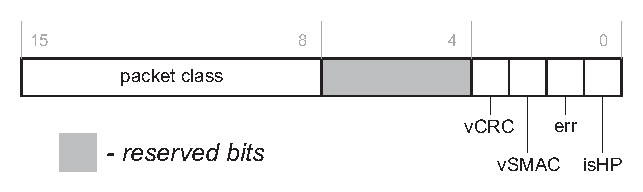
\includegraphics[width=.6\textwidth]{fig/status.pdf}
    \caption{Status word format}
  \end{center}
\end{figure}

\begin{itemize}
  \item[] \emph{isHP} - if \emph{1}, the frame is high priority
  \item[] \emph{err} - if \emph{1}, the frame contains an error
  \item[] \emph{vSMAC} - the frame contains a source MAC address (otherwise
    it will be assigned from WRPC configuration)
  \item[] \emph{vCRC} - the frame contains a valid CRC checksum
  \item[] \emph{packet class} - the packet class assigned by the classifier
    inside WRPC MAC module
\end{itemize}

OOB data is used for passing the timestamp-related information for the incoming and 
outgoing Ethernet frames. Each frame received from a physical link is
timestamped inside the WRPC and this value is passed as Rx OOB
data. On the other hand, for each transmitted frame the Tx timestamp can be read
from the Tx Timestamping Interface (section \ref{sec:txts}) together with a unique
frame number assigned in Tx OOB. Therefore, the format of OOB differs between Rx
and Tx frames.\\

{\bf Tx OOB format} (figure \ref{fig:fabric_adv:tx_oob}):

\begin{figure}[ht]
  \begin{center}
    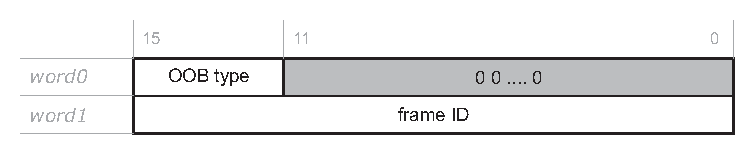
\includegraphics[width=.7\textwidth]{fig/oob_tx.pdf}
    \caption{Tx OOB data format}
    \label{fig:fabric_adv:tx_oob}
  \end{center}
\end{figure}

\begin{itemize}
  \item[] \emph{OOB type}: "0001" means Tx OOB
  \item[] \emph{frame ID}: ID of the frame being sent. It is later output
    through the \emph{Tx Timestamping interface} to associate Tx timestamp with
    appropriate frame. Frame ID = 0 is reserved for PTP packets inside WRPC
    and cannot be used by user-defined modules.
\end{itemize}

{\bf Rx OOB format} (figure \ref{fig:fabric_adv:rx_oob}):
\begin{figure}[ht]
  \begin{center}
    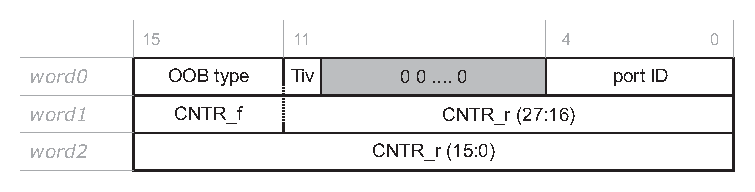
\includegraphics[width=.7\textwidth]{fig/oob_rx.pdf}
    \caption{Rx OOB data format}
    \label{fig:fabric_adv:rx_oob}
  \end{center}
\end{figure}

\begin{itemize}
  \item[] \emph{OOB type}: "0000" means Rx OOB
  \item[] \emph{Tiv}: timestamp invalid. When this bit is set to '1', the PPS
    generator inside WRPC is being adjusted which means the Rx timestamp is not
    reliable.
  \item[] \emph{port ID}: the ID of a physical port on which the packet was
    received. In case of WRPC, this field is always 0, because there is only one
    physical port available.
  \item[] \emph{CNTR\_f}: least significant bits of the Rx timestamp generated on
    the falling edge of the reference clock.
  \item[] \emph{CNTR\_r}: Rx timestamp generated on the rising edge of the reference
    clock.
\end{itemize}
